% Latex template: https://github.com/mqTeXUsers/Macquarie-University-Beamer-Theme

% Slide Masters:

% Title
% Text
% 2 column
% Full-image
% Bibliography
% Closing
 
\documentclass[aspectratio=169, 12pt]{beamer} % Aspect ratio
% https://tex.stackexchange.com/a/14339/5483 
% Possible values: 1610, 169, 149, 54, 43 and 32.
% 169 = 16:9

\PassOptionsToPackage{table}{xcolor}    %https://tex.stackexchange.com/a/5365/5483

\usetheme{macquarie}
\usepackage{multicol} % https://tex.stackexchange.com/a/396018/5483

\usepackage{svg} %https://github.com/mrpiggi/svg 

\usepackage[english]{babel}       % Set language
% \usepackage[utf8x]{inputenc}      % Set encoding
\usepackage{colortbl}
\mode<presentation>           % Set options
{
  \usetheme{default}          % Set theme
  \usecolortheme{default}         % Set colors
  \usefonttheme{default}          % Set font theme
  \setbeamertemplate{caption}[numbered] % Set caption to be numbered
}

% Uncomment this to have the outline at the beginning of each section highlighted.
%\AtBeginSection[]
%{
%  \begin{frame}{Outline}
%    \tableofcontents[currentsection]
%  \end{frame}
%}

\usepackage{graphicx}         % For including figures
\usepackage{booktabs}         % For table rules
\usepackage{hyperref}         % For cross-referencing


\usepackage{enumitem} % https://tex.stackexchange.com/a/2292/5483

%https://tex.stackexchange.com/a/371844/5483
\setbeamerfont{bibliography entry author}{size=\tiny}
\setbeamerfont{bibliography entry title}{size=\tiny}
\setbeamerfont{bibliography entry location}{size=\tiny}
\setbeamerfont{bibliography entry note}{size=\tiny}
\setbeamerfont{bibliography item}{size=\tiny}

%https://tex.stackexchange.com/q/333587/5483
%TODO SHAWN REPLACE OSF URL
%\setbeamertemplate{footline}{\strut~\texttt{https://osf.io/v5jp7/}\hfill\insertframenumber~/~\inserttotalframenumber\strut~~~}

\title{Seven years of FAIMS Mobile} % Presentation title
\author{Shawn A Ross | Brian Ballsun-Stant}               % Presentation author
\institute{Faculty of Arts}         % Author affiliation
\date{\today}                 % Today's date  
\begin{document}

% Title page
% This page includes the informations defined earlier including title, author/s, affiliation/s and the date
% \begin{frame}[noframenumbering]

\maketitle

  
% \end{frame}

% Outline
% This page includes the outline (Table of content) of the presentation. All sections and subsections will appear in the outline by default.
\begin{frame}{Strategies for field data capture infrastructure}
  \tableofcontents
\end{frame}

% The following is the most frequently used slide types in beamer
% The slide structure is as follows:
%
%\begin{frame}{<slide-title>}
% <content>
%\end{frame}

% Slides to speak to at CAA2019

% In-depth information for reference

\section{`Small data' infrastructure across the data lifecycle}

\begin{frame}{`Small data' research}
 \begin{figure}[H]
    \centering
        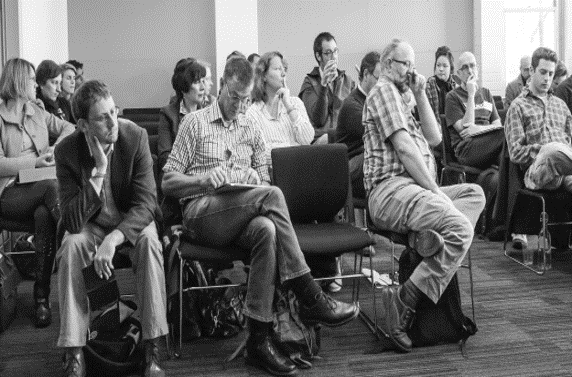
\includegraphics[height=.75\textheight]{figures/Archaeologists-standards.png}
        \caption{Archaeologists contemplate data standards (FAIMS Stocktaking, 2012)}
        \label{fig:figure7}
 \end{figure}
\end{frame}

\begin{frame}{Context: the challenge of `small data'}
    `Long tail' research: most field data is small data \cite{Borgman2015-rh}
    \begin{itemize}[label=\textbullet]
        \item Smaller scale; smaller communities; local control.
        \item Diverse questions, approaches, and methods.
        \item Heterogeneous data; variety of content, structure.
        \item Data and infrastructure emerge from fieldwork. 
        \item Relative lack of standards.
        \item Limited infrastructure and funding.
        \item Challenges associated with big(ger) data from photogrammetry, SfM, video, geophysics, etc., will exacerbate these problems.
    \end{itemize}
\end{frame}

\begin{frame}{The data lifecycle}
 \begin{figure}[H]
    \centering
        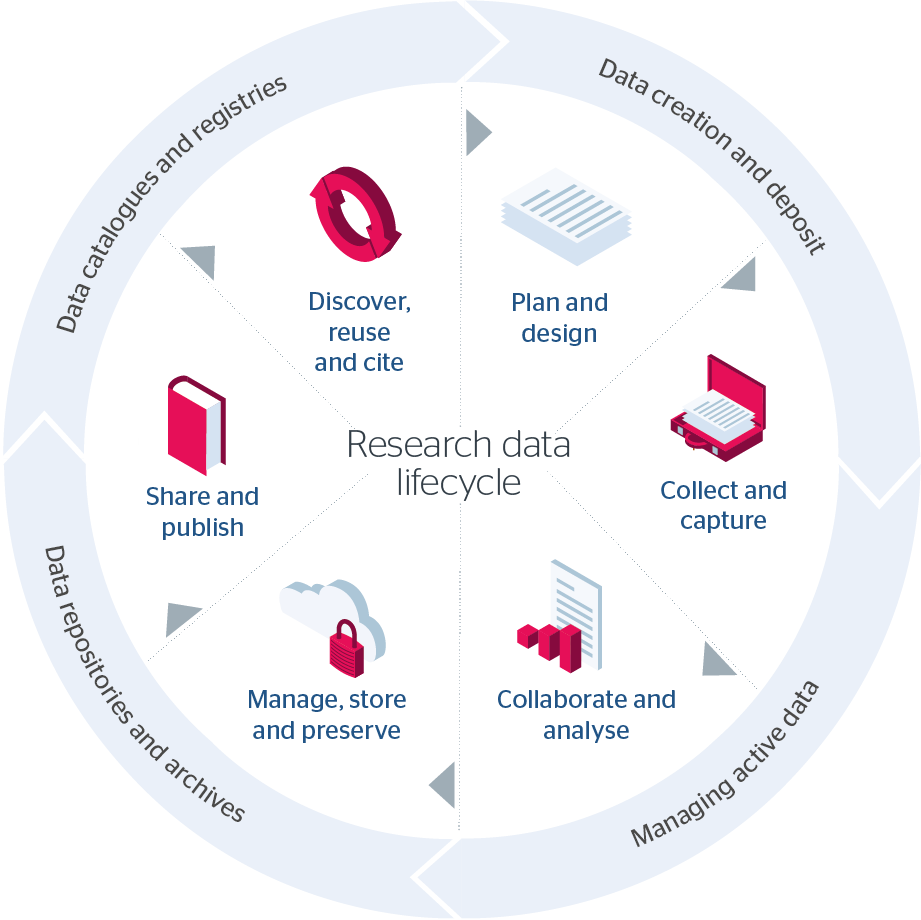
\includegraphics[height=.75\textheight]{figures/research-data-life-diagram.png}
        \caption{\cite{Jisc2018-gx} Image CC-BY-ND}
        \label{fig:figure9}
 \end{figure}
\end{frame}

\begin{frame}{Infrastructure across the data lifecycle}
    Consider the infrastructure needed to manage the three main phases of the data lifecycle
    \begin{itemize}[label=\textbullet]
        \item Publication (most mature): domain-specific repositories.
        \item Processing and analysis (less mature): project-level code \cite{Stewart_Lowndes2017-lj}, then Virtual Labs / Science Gateways, \cite{Alveo2019-tk}.
        \item Capture (least mature): most varied, needs to work offline under difficult conditions. Existing commercial solutions insufficient \cite{Bureau_of_Reclamation2017-xl}.
    \end{itemize}
\end{frame}


% Slides to speak to at WSU 5 June 2019

\section{The FAIMS approach: summary}

\begin{frame}{Research Specific}
 \begin{figure}[H]
    \centering
        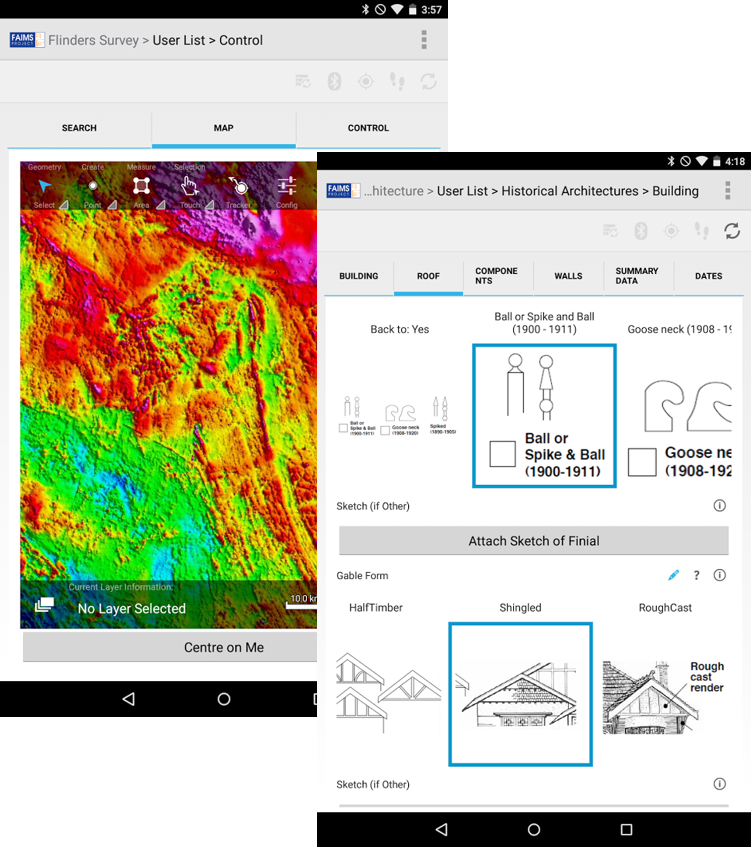
\includegraphics[height=.75\textheight]{figures/FAIMS-screenshots.png}
        \caption{FAIMS Mobile: GIS and `picture dictionaries'}
        \label{fig:FAIMS-mobile-screenshots}
 \end{figure}
\end{frame}


\begin{frame}{Generalised}
 \begin{figure}[H]
    \centering
        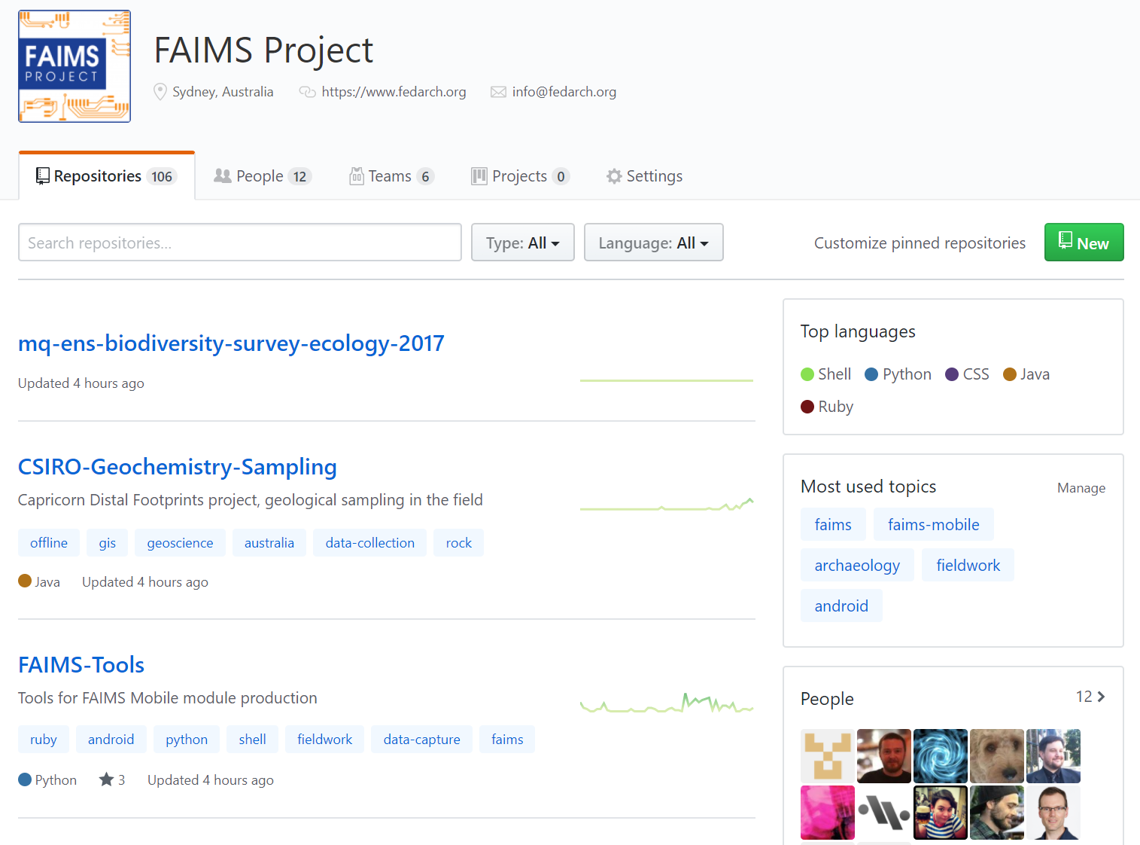
\includegraphics[height=.75\textheight]{figures/FAIMS-generalised.png}
        \caption{FAIMS Mobile customisations on GitHub}
        \label{fig:FAIMS-github}
 \end{figure}
\end{frame}

\begin{frame}{Modular and federated}
 \begin{figure}[H]
    \centering
        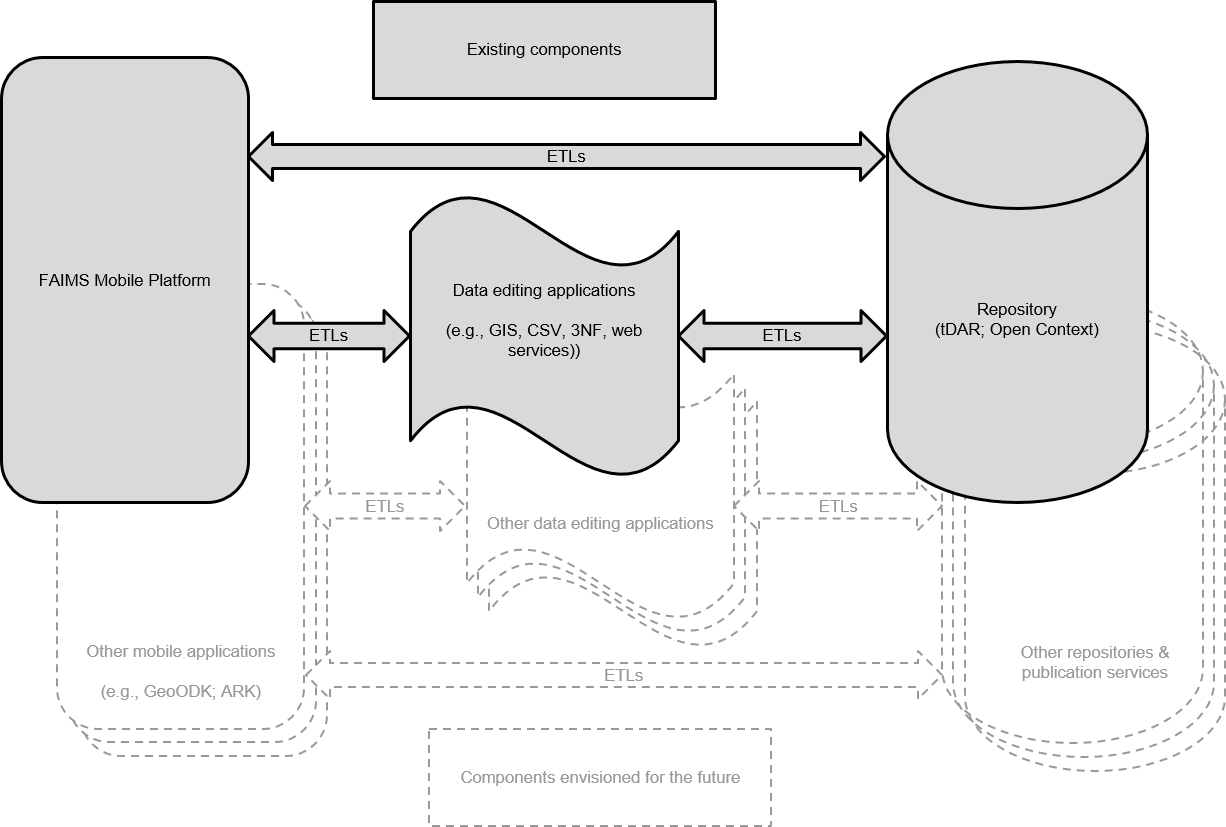
\includegraphics[height=.75\textheight]{figures/FAIMS-federated.png}
        \caption{FAIMS Mobile federation}
        \label{fig:FAIMS-federation}
 \end{figure}
\end{frame}

\begin{frame}{Open Source}
 \begin{figure}[H]
    \centering
        
\includegraphics[width=.75\textwidth]{figures/GPLv3_Logo.eps}
        \caption{FAIMS Mobile 'core' code is GPLv3; 'module' (customisation) code is also open; everything is on GitHub}
        \label{fig:FAIMS-github-OSS}
 \end{figure}
\end{frame}

\begin{frame}{Key research-specific FAIMS Mobile features}
    \begin{itemize}[label=\textbullet]
        \item Fundamentally customisable (interpreter + definition files).
        \item Tightly binds structured, geospatial, multimedia, and free text data.
        \item Works offline.
        \item Automated bi-directional synchronisation using local or online server
        \item Record history: append-only datastore, versioning, rollback.
        \item Mobile GIS.
        \item Connects to internal and external sensors, Bluetooth / USB devices.
        \item Multilingual.
        \item Granular help.
        \item Granular metadata / uncertainty.
        \item Generalised export.
        \item `Hooks’ for data interoperability, Open Linked Data approaches.
    \end{itemize}
\end{frame}

\begin{frame}{FAIMS publications}
      \begin{itemize}[label=\textbullet]
        \item \cite{Sobotkova2018-al}
        \item \cite{Ballsun-Stanton2018-zd}
        \item \cite{VanValkenburgh2018-hv}
        \item \cite{sobotkova2016-mx}
        \item \cite{Ross2015-ph} 
        \item \cite{Sobotkova2015-lq}
        \item \cite{Ross2013-hi}
    \end{itemize}
\end{frame}

\begin{frame}{Thank you!}

%This presentation is available at:
%\texttt{https://osf.io/v5jp7/}

Source code for this presentation is available at: 
\texttt{https://github.com/ saross/Ross-FAIMS-intro}.

FAIMS Project software and documentation can be found at:
\texttt{https://github.com/faims}.

This work is licensed under a Creative Commons Attribution 4.0 International License.

\end{frame}

% In-depth information for reference
\section{The FAIMS approach: in-depth}

\begin{frame}{Introduction to the FAIMS Project}
    \begin{itemize}[label=\textbullet]
        \item The Field Acquired Information Management Systems (FAIMS) Project began in 2012 as a national Australian information infrastructure project in archaeology.
        \item Developed FAIMS Mobile for field data capture \cite{Ballsun-Stanton2018-zd}.
        \item Use expanded beyond archaeology to geoscience, ecology, ethnography, linguistics, oral history.
        \item Has been customised for over 50 workflows at more than 30 projects. 
        \item Data and workflow modelling for these customisations provided deep insights into field data capture and the infrastructure needed to support it.
    \end{itemize}
\end{frame}

\begin{frame}{FAIMS Mobile software}
 \begin{figure}[H]
    \centering
        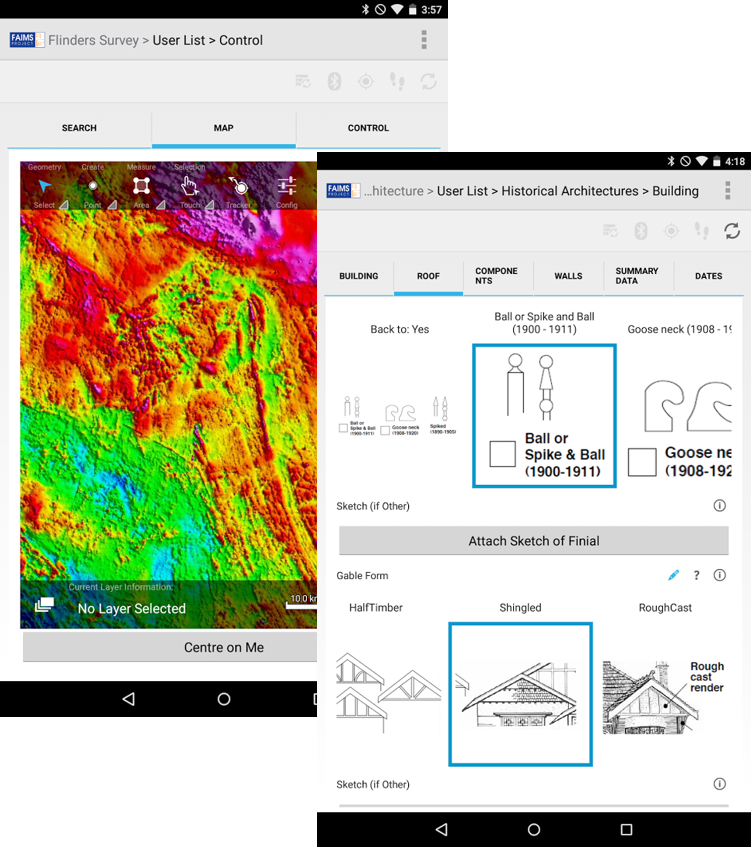
\includegraphics[height=.75\textheight]{figures/FAIMS-screenshots.png}
        \caption{FAIMS Mobile: GIS and `picture dictionaries'}
        \label{fig:figure10}
 \end{figure}
\end{frame}

\begin{frame}{Field data capture infrastructure: a manifesto}
    \begin{itemize}[label=\textbullet]
        \item Our domains deserve research-specific software.
        \item Diverse practices and limited resources require generalised software.
        \item Do one thing well with modular and federated software (but slice the pie thoughtfully).
        \item Open-source software supports open research and has other advantages (but is difficult to sustain). 
        \item Scope requirements carefully.
        \item Invest in outreach and engagement.
    \end{itemize}
\end{frame}

\begin{frame}{Research specific}
    Field research needs (and deserves) research-specific software, contra \cite{Roosevelt2015-kd}.
      \begin{itemize}[label=\textbullet]
        \item Most commercial / mass-market software does not meet research needs.
        \item Risk of lock-in, unwelcome changes to features or business models, and product discontinuation.
    \end{itemize}
    Compare ecology: TERN, ALA, Biocollect, and associated research clouds \cite{Tern2019-sp, Ala2019-by, Ala2019-cb}.
\end{frame}

\begin{frame}{Generalised (not generic or bespoke)}
  Commercial software doesn't meet our needs, and bespoke development is too expensive and usually unsustainable.
      \begin{itemize}[label=\textbullet]
        \item Generalised software can be deeply customised to accommodate our diverse data types, data models, workflows, etc.
        \item The code used to customise it describes the data model and workflow.
        \item Customisations can be published and re-deployed trivially.
        \item Can deliver research-grade software affordably.  
    \end{itemize}
    FAIMS Mobile cost perhaps 3x a single bespoke application, but has been customised 50x. Customisation cost is 1/10th bespoke, and still <1/2 even if `core' platform development costs are amortised across projects.
\end{frame}

\begin{frame}{Generalised: customise using code}
 \begin{figure}[H]
    \centering
        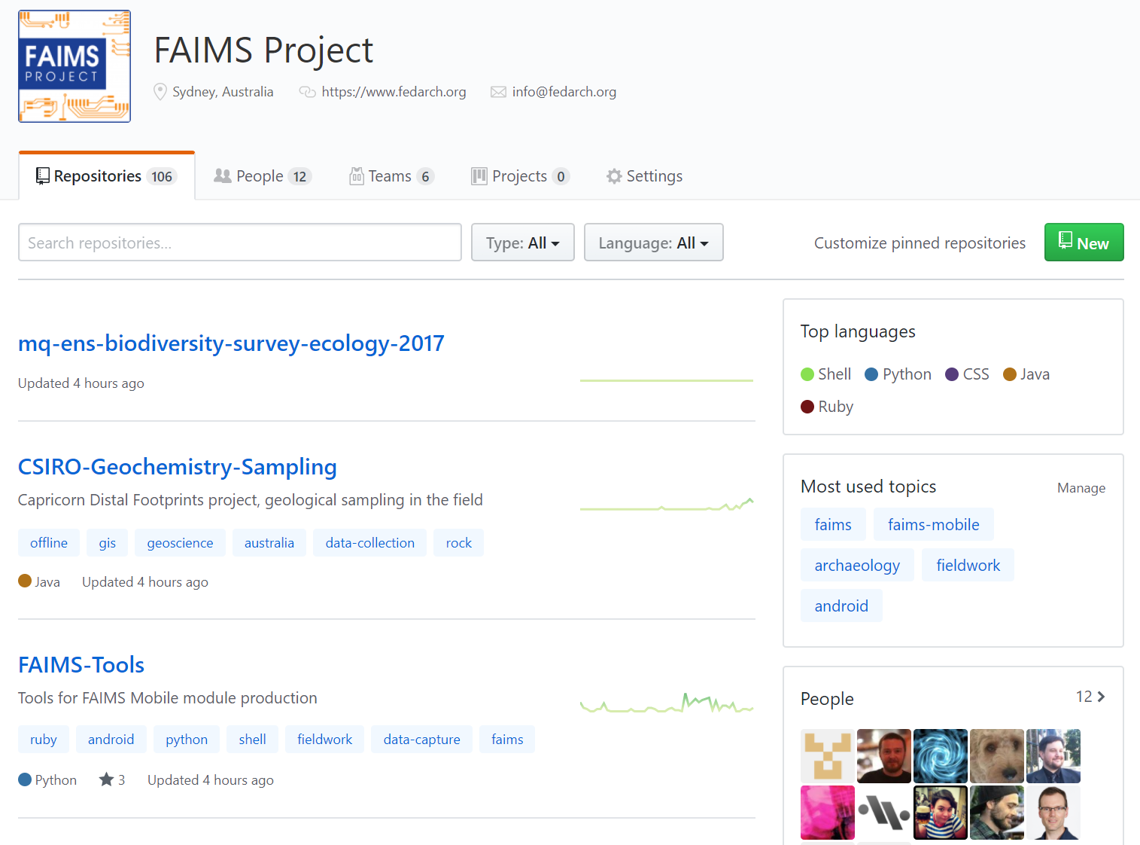
\includegraphics[height=.75\textheight]{figures/FAIMS-generalised.png}
        \caption{FAIMS Mobile customisations (XML files, mostly) on GitHub}
        \label{fig:figure11}
 \end{figure}
\end{frame}

\begin{frame}{Modular and federated}
  Do one thing well.
      \begin{itemize}[label=\textbullet]
        \item Identify other infrastructure in the domain and interoperate with it (via ETLs or APIs).
        \item It is better to divide by data-lifecycle phase rather than data type, since (1) our data is so integrated and (2) field data capture poses unique challenges.
    \end{itemize}
\end{frame}

\begin{frame}{Modularise by data lifecycle phase}
 \begin{figure}[H]
    \centering
        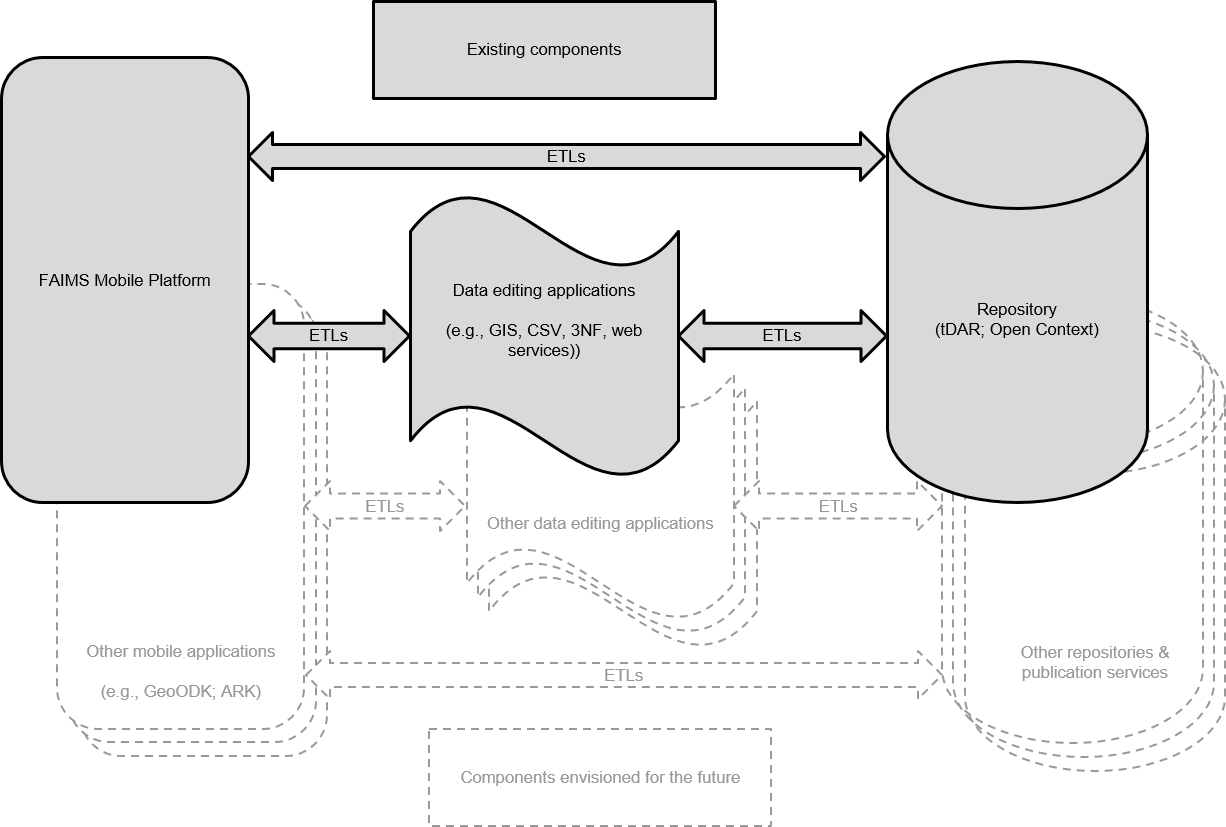
\includegraphics[height=.75\textheight]{figures/FAIMS-federated.png}
        \caption{FAIMS Mobile federation strategy}
        \label{fig:figure13}
 \end{figure}
\end{frame}

\begin{frame}{Open source?}
  Open source has advantages but is difficult to sustain.
      \begin{itemize}[label=\textbullet]
        \item Emerging open research principles strongly prefer OSS as opposed to proprietary ‘black boxes’.
        \item Transparency and reusability (esp. customisation code).
        \item Ability to hand off from one organisation to another (esp. `core' platform code).
        \item Ability to fork code prevents lock-in and mitigates unwelcome decisions by software developers.
        \item BUT OSS business models are hard to scale and rely on occasional injections of grant or institutional funding.
    \end{itemize}
\end{frame}

\begin{frame}{Scope carefully}
  Talk to a wide range of potential users, seeking facts not opinions.
      \begin{itemize}[label=\textbullet]
        \item Don’t ask researchers what they think, ask them what they have done - what software they have adopted and why, and what problems they have expended resources to solve. 
        \item ‘Lean startup’ methodology very useful, based around  testing of ideas through interviews with potential users \cite{Strategyzer_AG2019-uu}.
        \item In our case, we over-invested in mobile GIS and under-invested in usability (especially a GUI for customisation).
    \end{itemize}
\end{frame}

\begin{frame}{Spend on outreach and engagement}
  If you build it they will not come; people can't use technologies they don't know about.
      \begin{itemize}[label=\textbullet]
        \item As per industry standards, dedicate at least 30\% of any information infrastructure budget to outreach and engagement (sales and marketing). 
        \item Typical academic outreach (journal articles, conference presentations, workshops, even booths at major conferences) are not enough.
    \end{itemize}
\end{frame}

\section{From current practice to better practice}

\begin{frame}{Challenges and paths forward}
  How do we get from where we are now to where we want to be?
      \begin{itemize}[label=\textbullet]
        \item Understand the evolving expectations of transparent research. 
        \item Look past desktop software (Excel, ARCGIS, Filemaker, Access, etc.).
        \item Rally around emerging research- and domain-specific solutions (even if imperfect).
        \item Overcome `not invented here'; you don't need a bespoke solution.
        \item Budget for `ground-up' transparency (data and code). Up-front costs will be high but offer longer-term payoffs (in costs, time, and quality).
        \item Implement (and budget for) fundamental good practice in data and code management before other technologies.
        \item Improve research design (prioritise approach over methods) \cite{Muthukrishna2019-kt, Hole1973-cy}
    \end{itemize}
\end{frame}

% \bibliographystyle{apalike}
 
% Adding the option 'allowframebreaks' allows the contents of the slide to be expanded in more than one slide.
% The "1" comes from the outer theme"

\section{References}

% \begin{frame}[allowframebreaks]{References}
  
%   \bibliography{references}
%   \bibliographystyle{apalike}
% \end{frame}

\begin{multicols}{2}[]
\bibliography{references}
\bibliographystyle{apalike}
\end{multicols}

\end{document}
